% !TeX spellcheck = en_US
\documentclass[french]{yLectureNote}

\title{Mathématiques}
\subtitle{Langage mathématique}
\author{Paulhenry Saux}
\date{\today}
\yLanguage{Français}

\professor{C.Dartyge}

\usepackage{graphicx}%----pour mettre des images
\usepackage[utf8]{inputenc}%---encodage
\usepackage{geometry}%---pour modifier les tailles et mettre a4paper
%\usepackage{awesomebox}%---pour les boites d'exercices, de pbq et de croquis ---d\'esactiv\'e pour les TP de PC
\usepackage{tikz}%---pour deiffner + d\'ependance de chemfig
\usepackage{tkz-tab}
\usepackage{chemfig}%---pour deiffner formules chimiques
\usepackage{chemformula}%---pour les formules chimiques en \'equation : \ch{...}
\usepackage{tabularx}%---pour dimensionner automatiquement les tableaux avec variable X
\usepackage{awesomebox}%---Pour les boites info, danger et autres
\usepackage{menukeys}%---Pour deiffner les touches de Calculatrice
\usepackage{fancyhdr}%---pour les en-t\^ete personnalis\'ees
\usepackage{blindtext}%---pour les liens
\usepackage{hyperref}%---pour les liens (\`a mettre en dernier)
\usepackage{caption}%---pour la francisation de la l\'egende table vers Tableau
\usepackage{pifont}
\usepackage{array}%---pour les tableaux
\usepackage{lipsum}
\usepackage{yFlatTable}
\usepackage{multicol}
\newcommand{\Lim}[1]{\lim\limits_{\substack{#1}}\:}
\renewcommand{\vec}{\overrightarrow}
\begin{document}

\titleOne

	\chapter{Introduction au raisonnement }
\section{Vocabulaire}
\infoInfo{Paradoxe du tas de sable}{A partir de combien de grain on considère que c'est un tas de sable. Si on enlève un grain, peut on dire que c'est toujours un tas ? Problème de langage et de définition}
\subsection{Ensemble}
\begin{theorem}[Ensemble]
Un ensemble est constitué d'éléments et est défini par une relation d'appartenance
\end{theorem}
Soit E un Ensemble. Il est bien défini si $\forall$ x on peut dire sans ambiguïté si $x\in E$ (x appartient à E) Dans le cas contraire, il n'appartient pas.

\warningInfo{}{Un ensemble n'est jamais élément de lui même. Conséquence : La collection de tous les ensemble n'est pas un ensemble (car il s'appartiendrait à lui-m\^eme}
Exemples : $\mathbb{N}, \mathbb{C}$.
\subsection{Éléments de logique propositionnelle}
\subsubsection{Assertions}
Assertion : Une phrase grammaticalement correcte dont on peut dire sans ambiguïté si elle est vraie ou fausse
\checkInfo{Exemples}{Exemple 1 : P : ``Les élèves du TDA2 sont au nombre de 37'' P est fausse.

Exemple 2 : P : ``Je mens'' n'est pas une assertion mais un paradoxe

Exemple 3 : $1+1=2$ est une assertion}

\subsubsection{Opérations logique}

Négation : $\neg$

Et : $\wedge$

Ou : $\vee$

$\neg P$ est vrai si $P$ est faux

$\neg P$ est faux si $P$ est vrai\marginCritical{Le contraire de tous/pour tous est au moins un}

\checkInfo{Exemple}{$P$ : Tous les chevaux de Martine sont noirs

$\neg P$ : Au moins un des chevaux n'est pas noirs

$Q$ : Au moins un des étudiant n'a pas de téléphone

$\neg Q$ : Tous les étudiants ont un téléphone}

	\begin{tabular}{_c^c^c^c^c^c^c}
		\tableHeaderStyle%
P & Q & P et Q& P ou Q & P $\Rightarrow$ Q& P $\iff$ Q &$\neg P$\\
V & V & V & V & V & V &F\\
V & F & F & V & F & F&F\\
F & V & F & V & V & F&V\\
F & F & F & F & V & V&V\\
	\end{tabular}


\criticalInfo{Attention si La première assertion est fausse}{
Paris n'est pas la capitale de France (F) $\Rightarrow$ Tous les élèves ont une voiture (V) : Assertion vraie

Paris est la capitale de la France (V) $\Rightarrow$ Tous les étudiants sont en bleu. (F) : Assertion fausse}


On suppose maintenant P ou $\neg$ P. Il faut montrer que si P est vrai alors Q est vrai.

\subsubsection{Règles de calcul}
$\neg (\neg P) = P$

$\neg(P \wedge Q) = \neg P \vee \neg Q$

$P\iff Q = \neg P \vee Q$

Attention : $\neg (P \Rightarrow Q) = P \wedge \neg Q$

\checkInfo{Exemple}{
Assertion : $x\in \mathbb{R}$ $\Rightarrow x$ a une racine

Le contraire est : (x$\in \mathbb{R}$) $\wedge$ (x n'a pas de racine)}

\subsubsection{Contraposée}
Contraposé : $(P \Rightarrow Q) \iff (\neg Q \Rightarrow \neg P)$


$\forall x,y \in R,\: x\neq y \Rightarrow x^3\neq y^3$ $\iff x^3=y^3 \Rightarrow x=y$

\subsubsection{Prédicat}
$P(x_1\dots x_r)$ est un prédicat si c'est une phrase correcte qui dépend de variables et dont on peut dire la valeur de vérité pour tout k-uplet donné.\marginTips{(Assertion sauf que l'on a pas défini les variables)}

\subsubsection{Quantificateurs}
Quantificateur universels : $\forall$ = Pour tout

Quantificateur d'existence : $\exists$ = Il existe au moins un

Ils transforment un prédicat en assertion

\subsubsection{Proposition}
$\neg (\forall x, P(x)) = \exists x, \neg P(x)$

$\neg(\exists x, P(x)) = \forall x, \neg P(x)$

Ex 1.5

\begin{center}
Fin Séance 1
\end{center}

\yOrnament
\section{Raisonnements}
\subsection{Par l'absurde}
\subsubsection{Tautologie et contradiction}

\begin{theorem}[Tautologie]
Formule propositionnelle toujours vraie
\end{theorem}

Ex : $P \vee \neg P$

\begin{theorem}[Contradiction]
Formule propositionnelle toujours fausse
\end{theorem}

Ex : $P \wedge \neg P$
\subsubsection{Fonctionnement}
On cherche à démontrer une propriété $P$ en supposant $\neg P$. On poursuit le raisonnement jusqu'à arriver à une contradiction. Comme les mathématiques sont non contradictoire, l'hypothèse de départ est fausse. Donc $\neg P$ est fausse, D'où $P$.

\checkInfo{Exemple}{Montrer que $\sqrt{2} \notin \mathbb{Q}$, en effectuant un raisonnement par l'absurde.

Je suppose que $\sqrt{2} \in \mathbb{Q}$

Donc $\exists a \in \mathbb{N}, \exists b \in \mathbb{N}^*, \sqrt{2} = \frac{a}{b}, PGCD(a,b) = 1$.

$\sqrt{2} = \frac{a}{b} \Rightarrow 2b^2 = a^2$.

Donc $2|2b^2$, donc $2|a^2$ et $2|a$. Donc $\exists a'$ tq $a = 2a'$.

Donc $2b^2 = a^2 = 4a'^2 \Rightarrow b^2 = 2a'^2$. Donc $2|b^2$ et $2|b$. Donc Le PGCD est de 2 et non de 1, contradiction. }

\subsection{Par récurrence}
On veut démontrer des assertions où $n\in \mathbb{N}$.

\begin{theorem}[Proposition]
Si $(P(0)$ et $(\forall n\in \mathbb{N}, P(n) \Rightarrow P(n+1)$, alors $\forall n\in \mathbb{N}, P(n)$.
\end{theorem}

\checkInfo{Exemple : Montrer que $\forall n \in \mathbb{N}, n < 2^n$}{

Soit $H(n) =  n < 2^n$.

Je démontre $H(n)$ par récurrence sur $n\in \mathbb{N}$.

Initialisation

$H(0) : 0<2^0 = 1$, donc $H(0)$.

Hérédité

On suppose $H(n)$, montrons $H(n+1)$, ie $n+1<2^{n+1}$.

D'après $H(n)$, $n+1 < 2^n + 1$. Or $n<2^n$, d'où $ n+1 < 2^n + 2^n = 2^{n+1}$.

Donc $H(n+1)$ et $H(n) \Rightarrow H(n+1)$.

Conclusion
\begin{itemize}
 \item $H(0)$
 \item $\forall n \in \mathbb{N}, H(n) \Rightarrow H(n+1)$
\end{itemize}

Donc $\forall n \in \mathbb{N}, H(n) : n<2^n$.

}
\subsection{Récurrence à 2 pas}
\begin{theorem}[Déf]
Si $(P(0)\wedge P(1)) \wedge (\forall n \in \mathbb{N}, P(n) \wedge P(n+1) \Rightarrow P(n+2))$, alors $P(n)$.
\end{theorem}
\subsection{Récurrence forte}
\begin{theorem}[définition]
Si $P(0) \wedge (\forall n \in \mathbb{N}, [\forall \mathbb{R} \in \{0,\dots,n\}, P(k) \Rightarrow P(n+1)])$, alors $P(n) \forall n \in \mathbb{N}$.
\end{theorem}
Ex 1.11 : Produit de plusieurs entiers impairs.
Ex 1.12 : Récurrence\marginCritical{Utilisation des signes sigma pour somme et grand pi pour produit}
\section{Théorie des ensembles}
\begin{theorem}[Égalité d'Ensemble]
Soit E et F 2 ensembles. Ils sont égaux ssi $\forall x, x \in E \iff x \in F$. On écrit alors E = F.
\end{theorem}

\begin{theorem}[Inclusion]
E est inclu dans F ssi $\forall x, x \in E \Rightarrow x \in F$. On écrit alors $E \subset F$. E est un sous ensemble de F
\end{theorem}



Remarque : $E \not\subset F \iff \exists x, x \in E \wedge x \notin F$

\begin{axiom}[Axiome]
Il existe un ensemble appelé ensemble vide  noté $\varnothing$, tel que $\forall x, x \notin \varnothing$.
\end{axiom}

\begin{axiom}[Unicité de l'ensemble vide]
Cet Ensemble est unique
\end{axiom}
Preuve : Supposons qu'il existe 2 ensembles vides, notés E et F.

Montrons que E = F.

$\forall x, x\notin E \Rightarrow x \notin F$.

Par contraposé : $\neg (x\in F) \Rightarrow \neg(x \in E)$. $\iff (x \in F \Rightarrow x \in E)$. De la même façon en permutant les r\^oles de E et F, on a $x \in E \Rightarrow x \in F$ et $E = F$.

\begin{axiom}[Parties de E]
L'ensemble de tous les sous-ensembles d'un ensemble E est un Ensemble E, que l'on note P(E)
\end{axiom}

\begin{axiom}[Collection des x de E qui vérifient P(x)]
Soit E un Ensemble, Soi P(x) un prédicat défini sur E, alors la collection des x de E qui vérifient P(x) est un ensemble. On le note $(x, x \in E \wedge P(n)$
\end{axiom}

\begin{theorem}[Conséquence]
Soit E et F 2 ensembles.

l'intersection de E et F, noté $(E \cap F) = \{x, x \in E \wedge x\in F\}$ est un ensemble.

La réunion de E et F est défini par $(E \cup F) = \{x, x \in E \vee x\in F\}$ est un ensemble complémentaire F dans E

$E \backslash F = \{x \in E, x \notin F\}$ est un ensemble.
\end{theorem}

\begin{axiom}[Produit cartésien]
Soit E et F 2 ensembles. On appelle produit cartésien de E et F l'ensemble des couples $E\times F = \{(x;y), x\in E, y \in F\}$.
\end{axiom}

\begin{theorem}[Propriété]
$\varnothing \subset E$ pour tout Ensemble. $\forall x, x \notin E \Rightarrow x \notin \varnothing$ et par contraposé : $x\in \varnothing \Rightarrow x \in E$.
\end{theorem}

\checkInfo{Exemples}{
$E = \{1.2\}$

$P(E) = \{\varnothing; \{1\}; \{2\}; \{1,2\}\}$

$P(\varnothing) = \{\varnothing\}$

$P(P(\varnothing)) = \{\varnothing, \{\varnothing\}\}$}

\begin{center}
Fin Séance 2
\end{center}

\yOrnament
\tipsInfo{Syntaxe pour $A\times B$}{
$\{(1,1);(1,5)\}$
}
Démontrer une inclusion : Démontrer que $\forall x, x\in B \Rightarrow x \in A$.
\section{Propriétés de l'intersection}
Soit E un ensemble, A et B deux parties de E.

$A \cap B = \{x\in E, x\in A \wedge x\in B\}$.

$A \cup B = \{x\in E, x\in A \vee x\in B\}$.

\begin{theorem}[Def]
Le complémentaire de A dans E, noté $\bar{A}$ est l'ensemble défini par $x\in \bar{A} \iff x \notin A$. Ainsi, $\bar{A} = \{x\in E, x\notin A\}$.
\end{theorem}
\begin{theorem}[Propriétés]
$\overline{A\cap B} = \bar{A} \cup \bar{B}$.

$\overline{A\cup B} = \bar{A} \cap \bar{B}$.

$A\cap(B\cup C) = (A\cap B)\cup (A\cap C)$.

$A\cup (B\cap C) = (A\cup B)\cap (A\cup C)$.

$\bar{\varnothing} = E$.

$\bar{E} = \varnothing$.

$\bar{\bar{A}} = A$.
\end{theorem}


Exemple : $x\in \bar{A\cap B} \iff \neg(x\in A\cap B) \iff \neg(x\in A \wedge x \in B) \iff \neg x\in A \vee \neg x\in B \iff x\notin A \vee x\notin B \iff x\in \bar{A} \vee x\in \bar{B} \iff ((x\in \bar{A}) \vee (x\in \bar{B}))$.

\begin{theorem}[Definition]
Soit I un ensemble, et $\forall i\in I$, soit $F_i$ un ensemble.

$F = (F_i, i\in I)$.

I est appelé ensemble des index.

$\forall x, x \bigcap\limits_{i\in I} F_i \iff \forall i \in I, x \in F_i$.

$\bigcap\limits_{i\in I} = \{x, x\in F_i, \forall i \in I\}$.

$x\in \bigcup\limits_{i\in I} F_i \iff \exists i\in I, x \in F_i$.

$\bigcup\limits_{i\in I} = \{x, \exists i\in I, x\in F_i\}$.
\end{theorem}
Exemples :

$\bigcup\limits_{n\in \mathbb{N}} [n, n+1[ = [0,+\infty[$

$\bigcap\limits_{n\in \mathbb{N}} [n, n+1[ = \varnothing$

$\bigcap\limits_{n\in \mathbb{N}^*} [-n, n[ = \varnothing$

$\bigcap\limits_{n\in \mathbb{N}^*} [-n, n] = [-1,1]$

$\bigcap\limits_{n\in \mathbb{N}^*} [-\frac{1}{n}, \frac{1}{n}] = \{0\}$\marginCritical{Le contenu de l'ensemble, ici celui du singleton 0 n'a pas besoin d'appartenir à l'ensemble de définition de $n$, ici $\mathbb{N}^*$.}

\section{Applications}
Soient E et F 2 ensembles non vides.
\subsection{Définition}
\begin{theorem}[Definition]
Une application f de E vers F, notée $f:E \rightarrow F$ est définie par la donnée d'un sous-ensemble $\Gamma_f$ de $E \times F$ qui vérifie la propriété : $\forall x \in E, \exists!y\in F, (x,y)\in \Gamma_f$. On écrit alors $y = f(x)$. $y$ est l'image unique de x. x est un antécédent de $y$.
\end{theorem}

Exemple : E = \{1,2,3,4\} et F = \{a,b,c\}

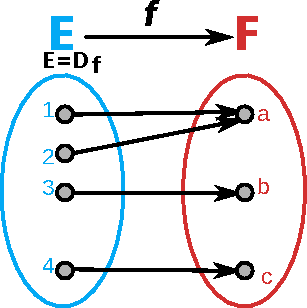
\includegraphics[scale=0.8]{app-def}

$\Gamma_f = \{(1,c);(2,b);(3,a);(4,b)\}$. On l'appelle le graphe de l'application. E est appelé ensemble de départ et F ensemble d'arrivée.

$f:E \rightarrow F$ est une application si tout élément de E a une unique image dans F.
\subsection{Injection, surjection, bijection}
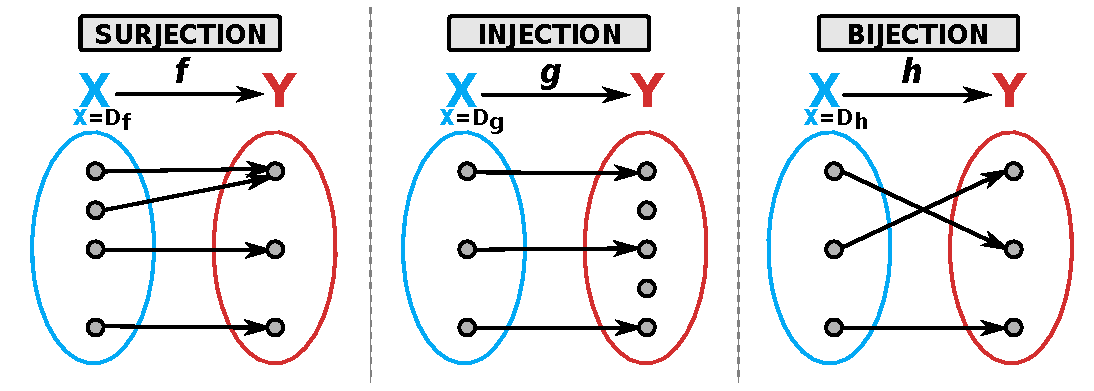
\includegraphics[scale=0.6]{application}
Soit $f:E\rightarrow F$ et $x\longmapsto f(x)$.

Soit $y\in F$. $\exists ? x\in E, y = f(x)$. On veut savoir le nombre de solution à cette équation.
\marginCheck{Si il y a :
\begin{itemize}
 \item au plus une solution, c'est injectif (Card(E) < ou > ? Card(F)
 \item au moins une solution, c'est surjectif,
 \item exactement une solution, c'est bijectif (Elles ont le m\^eme nombre d'élément, ensemble équipotent)
\end{itemize}}
\criticalInfo{Définitions à connaitre par coeur}{

\begin{theorem}[Surjectivité]
f est surjective de $E \rightarrow F \iff \forall y\in F, \exists x\in E, y = f(x) \iff$ tout élément de F admet au moins un antécédent dans E.
\end{theorem}
\begin{theorem}[Injectivité]
f est injective de $E \rightarrow F \iff (\forall x, x' \in E, x\neq x' \Rightarrow f(x)\neq f(x')) \iff (\forall x, x' \in E, f(x) = f(x') \Rightarrow x = x') \iff$ tout élément de F a au plus un antécédent dans E.
\end{theorem}
\begin{theorem}[Bijectivité]
f est bijective de $E \rightarrow F \iff (\forall x, x' \in E, \exists!x\in E, y=f(x) )\iff$ tout élément de F a un unique antécédent par f dans E. $\iff$ f est injective et surjective.
\end{theorem}

}
	\begin{tabular}{_l^l^l^l}
		\tableHeaderStyle%
		Fonction & Injective & Surjective\\
		$f: \mathbb{R} \to \mathbb{R}: x \mapsto x^2$ & Non & Non\\
		$f: \mathbb{R} \to \mathbb{R}: x \mapsto 2x$ & Oui & Oui \\
		$f: \mathbb{R}^+ \to \mathbb{R}^+: x \mapsto x^2$ & Oui & Oui\\
		$f: \mathbb{R}^+ \to \mathbb{R}: x \mapsto x^2$ & Oui & Non\\
		$f: \mathbb{R} \to \mathbb{R}^+: x \mapsto x^2$ & Non & Oui\\
		$f: \mathbb{R} \to [-1,1]: x \mapsto \sin(x), \cos(x)$ & Non & Oui\\
		$f: [0,2\pi[ \to [-1,1]: x \mapsto \sin(x)$ & Oui & Oui\\
	\end{tabular}
\begin{theorem}[Rappel de la définition de la composée d'une application]
Soient E,F,G 3 ensembles, Soit $f:E\rightarrow F$ $g:F\rightarrow G$

L'application $g\circ f$ est l'application définie par $g\circ f : E \rightarrow F \rightarrow G$ et $g\circ f : x \rightarrow f(x) \rightarrow g(f(x))$
\end{theorem}
\tipsInfo{Complément : Ensemble des éléments de E admettant une image}{
Soit $f : E \rightarrow F$ une application. On appelle antécédent d’un élément $y \in F$ par l’application $f$ tout élément $x \in E$ tel que $f (x) = y$ . L’ensemble des éléments de F qui admettent un antécédent par f est une partie de F appelée ensemble image ou image de f et notée $Im\:f$}

\tipsInfo{Complément : Application surjective sur $\mathcal{P}$}{
Il n’existe aucune application surjective d’un ensemble E sur $\mathcal{P}(E)$.}

\begin{theorem}[Définitions]
Soit $f:E \rightarrow F$ une application. Soit $A\subset E$, i.e $A\in P(E)$.

L'image directe de A, notée $f(A)$ est l'ensemble défini par : $f(A) = \{f(x),x\in A\} \subset F = \{y\in F, \exists x\in A, y=f(x)\}$.

Soit $B\subset F$. L'image réciproque de B pat f, notée $f^{-1}(B)$ est le sous-ensemble de E défini par $f^{-1}(B)=\{x\in E, f(x)\in B\}$ (= ``tiré en arrière de B'')
\end{theorem}
Exemple :

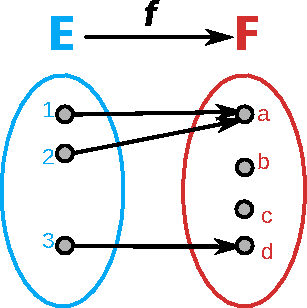
\includegraphics[scale=0.8]{app-ex}

Image directe

$f(E) = \{f(1),f(2),f(3)\} = \{a,d\}$

$f(\{1\}) = \{a\}$

$f(\{2,3\}) = \{a,d\}$

$f(\varnothing) = \varnothing$

Image réciproque

$f^{-1}(F) = E$ (toujours vrai, définition m\^eme d'une application)

$f^{-1}(\{a,d\}) = E$

$f^{-1}(\{c\}) = \varnothing$

$f^{-1}(\varnothing) = \varnothing$

$f^{-1}(\{a\}) = \{1,2\}$

\criticalInfo{Remarque}{
$f:E \rightarrow F$ est surjective si $f(E) = F$.}
\end{document}

